\documentclass{article}\usepackage[]{graphicx}\usepackage[]{color}
%% maxwidth is the original width if it is less than linewidth
%% otherwise use linewidth (to make sure the graphics do not exceed the margin)
\makeatletter
\def\maxwidth{ %
  \ifdim\Gin@nat@width>\linewidth
    \linewidth
  \else
    \Gin@nat@width
  \fi
}
\makeatother

\definecolor{fgcolor}{rgb}{0.345, 0.345, 0.345}
\newcommand{\hlnum}[1]{\textcolor[rgb]{0.686,0.059,0.569}{#1}}%
\newcommand{\hlstr}[1]{\textcolor[rgb]{0.192,0.494,0.8}{#1}}%
\newcommand{\hlcom}[1]{\textcolor[rgb]{0.678,0.584,0.686}{\textit{#1}}}%
\newcommand{\hlopt}[1]{\textcolor[rgb]{0,0,0}{#1}}%
\newcommand{\hlstd}[1]{\textcolor[rgb]{0.345,0.345,0.345}{#1}}%
\newcommand{\hlkwa}[1]{\textcolor[rgb]{0.161,0.373,0.58}{\textbf{#1}}}%
\newcommand{\hlkwb}[1]{\textcolor[rgb]{0.69,0.353,0.396}{#1}}%
\newcommand{\hlkwc}[1]{\textcolor[rgb]{0.333,0.667,0.333}{#1}}%
\newcommand{\hlkwd}[1]{\textcolor[rgb]{0.737,0.353,0.396}{\textbf{#1}}}%
\let\hlipl\hlkwb

\usepackage{framed}
\makeatletter
\newenvironment{kframe}{%
 \def\at@end@of@kframe{}%
 \ifinner\ifhmode%
  \def\at@end@of@kframe{\end{minipage}}%
  \begin{minipage}{\columnwidth}%
 \fi\fi%
 \def\FrameCommand##1{\hskip\@totalleftmargin \hskip-\fboxsep
 \colorbox{shadecolor}{##1}\hskip-\fboxsep
     % There is no \\@totalrightmargin, so:
     \hskip-\linewidth \hskip-\@totalleftmargin \hskip\columnwidth}%
 \MakeFramed {\advance\hsize-\width
   \@totalleftmargin\z@ \linewidth\hsize
   \@setminipage}}%
 {\par\unskip\endMakeFramed%
 \at@end@of@kframe}
\makeatother

\definecolor{shadecolor}{rgb}{.97, .97, .97}
\definecolor{messagecolor}{rgb}{0, 0, 0}
\definecolor{warningcolor}{rgb}{1, 0, 1}
\definecolor{errorcolor}{rgb}{1, 0, 0}
\newenvironment{knitrout}{}{} % an empty environment to be redefined in TeX

\usepackage{alltt}

\usepackage{rotating}
\usepackage{graphics}
\usepackage{latexsym}
\usepackage{color}
\usepackage{listings} % allows for importing code scripts into the tex file
\usepackage{wrapfig} % allows wrapping text around a figure
\usepackage{lipsum} % provides Latin text to fill up a page in this illustration (do not need it otherwise!)

% Approximately 1 inch borders all around
\setlength\topmargin{-.56in}
\setlength\evensidemargin{0in}
\setlength\oddsidemargin{0in}
\setlength\textwidth{6.49in}
\setlength\textheight{8.6in}

% Options for code listing; from Patrick DeJesus, October 2016
\definecolor{codegreen}{rgb}{0,0.6,0}
\definecolor{codegray}{rgb}{0.5,0.5,0.5}
\definecolor{codepurple}{rgb}{0.58,0,0.82}
\definecolor{backcolour}{rgb}{0.95,0.95,0.92}
\lstdefinestyle{mystyle}{
	backgroundcolor=\color{backcolour},   commentstyle=\color{codegreen},
	keywordstyle=\color{magenta},
	numberstyle=\tiny\color{codegray},
	stringstyle=\color{codepurple},
	basicstyle=\footnotesize,
	breakatwhitespace=false,         
	breaklines=true,                 
	captionpos=b,                    
	keepspaces=true,                 
	numbers=left,                    
	numbersep=5pt,                  
	showspaces=false,                
	showstringspaces=false,
	showtabs=false,                  
	tabsize=2
}

%"mystyle" code listing set
\lstset{style=mystyle}
%\lstset{inputpath=appendix/}


\title{Expenditures of Warwick and Monroe} 
\author{Kelso Quan}
\IfFileExists{upquote.sty}{\usepackage{upquote}}{}
\begin{document} 

\maketitle
\begin{center}
\Large{Abstract}
\end{center}
\qquad The study wanted to predict expenditures of New York cities, Warwick and Monroe. By gaining insight, the city council would like to know if its city will be spending more money  due to proposed construction of new housing projects and a possible growing population within city limits. While the cities are small to begin with, it is still a good idea to prepare for the future whether that be raising property taxes or looking for other sources of revenue. Looking into six predictor variables, a log linear trend was found between the resulting log transformed expenditure of the two cities and its six indicators. Furthermore, the pattern continued into the 2005 and 2025 predicted expenditures. It is noted that the predictions were made with a subset that required (log(pop) $>$ 8.3 \& log(dens) $>$ 4.5). Using the all six log transformed predictors, it was possible to come up with expenditure predictions. It was evident that there was a log positive trend with the six predictors (population, density, ''percent intergovernmental'', income, growth rate, and wealth), and the expenditures of both towns were going to increase over time. 

\section{Introduction}
\qquad In 1992, data was taken over a number of municipalities in New York state. By using the 914 observations taken, Warwick and Monroe city council should indeed plan for slightly higher expenditures by the city to keep up with the growing population possibly due to the planned housing projects. The $99\%$ confident intervals of each coefficient can be seen in Table \ref{coefficients}. These figures have been rounded. Please see the appendix for more exact numbers. The numbers in Table \ref{coefficients} have been transformed back. For example, every 1 unit (thousands) of wealth increased, the expenditure of Warwick and Monroe goes up by roughly \$1.50. 

Pint stands for ``Percent Intergovernmental'' which represents the percentage of revenue coming from state and federal grants subsidies. From Table \ref {predictions}, we have the prediction of expenditures in thousands. For exact figures, refer to the appendix. There is a slight positive linear trend while looking at the prediction intervals for Monroe, but it is noticeably more pronounce in Warwick's prediction of expenditures. 

\section{Methods}

\qquad The data was drawn from 916 municipalities in the state of New York in 1992. Two observations (i.e. Warwick and Monroe) were missing dataset. The purpose of the analysis is to predict expenditures of Warwick and Monroe from the data of 914 other municipalities. There was a municipality of interest which was included in the analysis. The observation 225 is influential point shown in figure \ref{cook}. While it is possible to remove this influential point, observation 225 was still a municipality of New York state. Removing it didn't change the model selection and thus was kept. The model selection and all analysis was done in R Studio to predict future expenditures.

\section{Results}

\subsection{Exploratory Data Analysis}

\qquad A boxcox transformation confirms that the response should be log transformed since $\lambda$ is near zero. Creating a histogram of the response variable expenditure shows a need for a log transformation. After the log transformation, the histogram of log-expenditure in figure \ref{response} shows lexpen is approximately normal. Taking a simple look at the predictor variables showed that they needed to be log transformed at least once before proceeding further. Histograms can be seen in figure \ref{regular} showed that there was heavy right skewness to all predictors before log transformations.  After log transformation, seen in figure \ref{transformed} showed nicer normality of each predictor. 

\quad Afterwards, the variable log expenditure was plotted against each of its predictor illustrated in figure \ref{scatterplots}. Each plot looked fairly linear. There didn't seem like an clear trends while plotting the residuals, thus no violation of homoscedasticity which can be seen in figure \ref{residuals}. There's no clear trends in the residuals and appeared to be random which is good news for linear regression. The QQ plot appears linear which suggest that the data is approximately normal after log transformations. 

\qquad In figure \ref{subset}, shows that there's a possible quadratic function, but the data could also be subsetted. This analysis focused on the subsetted data where log(pop) $>$ 8.3 and log(dens) $>$ 4.5 before more exploratory analysis was done. It is clear that the data must be subsetted. The blue lines shown in figure \ref{subset}, where the data should be subsetted.

\begin{figure}
  \begin{center}
    \caption{Log Dens and Log Pop before subsetting}
      \label{subset}
\begin{knitrout}
\definecolor{shadecolor}{rgb}{0.969, 0.969, 0.969}\color{fgcolor}
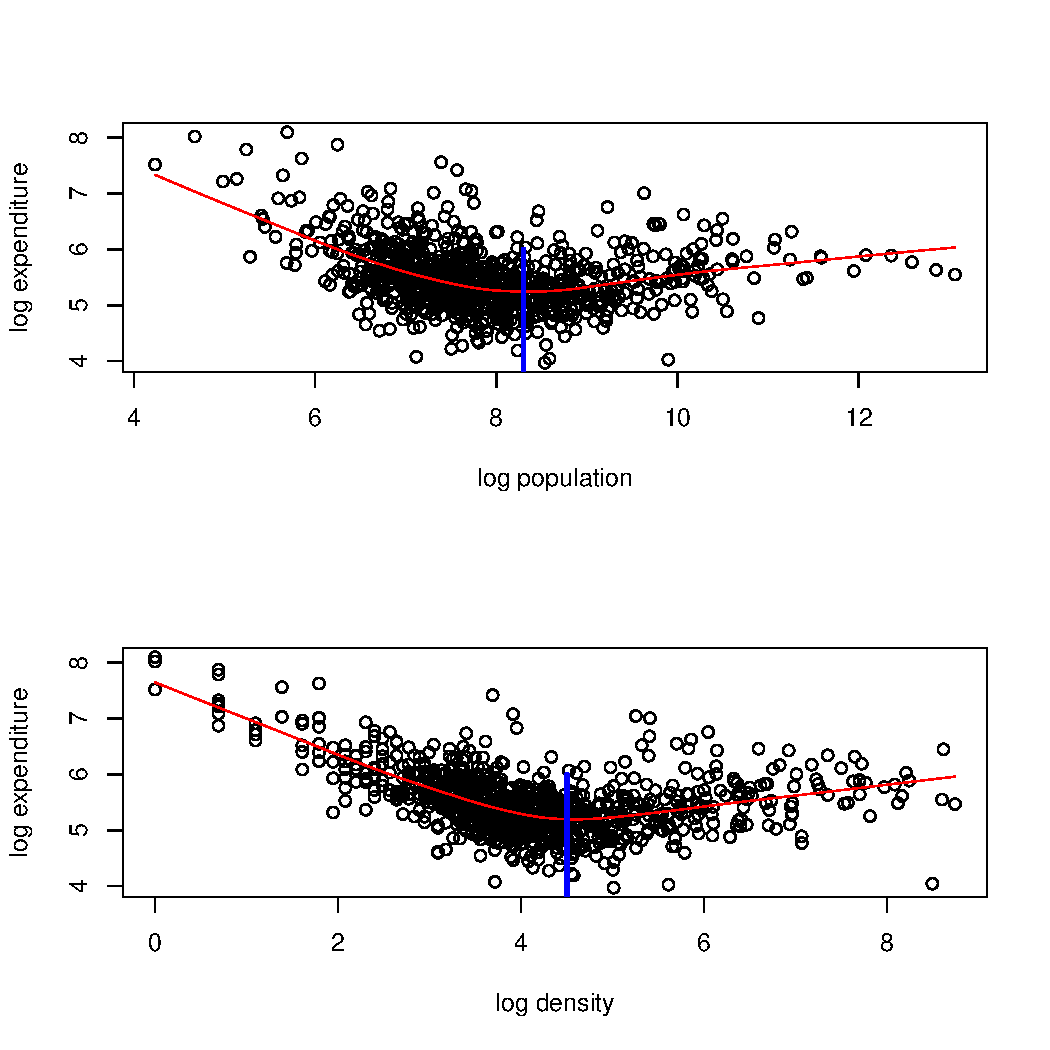
\includegraphics[width=0.5\linewidth]{figure/Reason_for_subsetted_data-1} 

\end{knitrout}
  \end{center}
\end{figure}

\begin{figure}
\begin{center}
\caption{Log Transforming Response Variable: Expenditures}
\label{response}
\begin{knitrout}
\definecolor{shadecolor}{rgb}{0.969, 0.969, 0.969}\color{fgcolor}
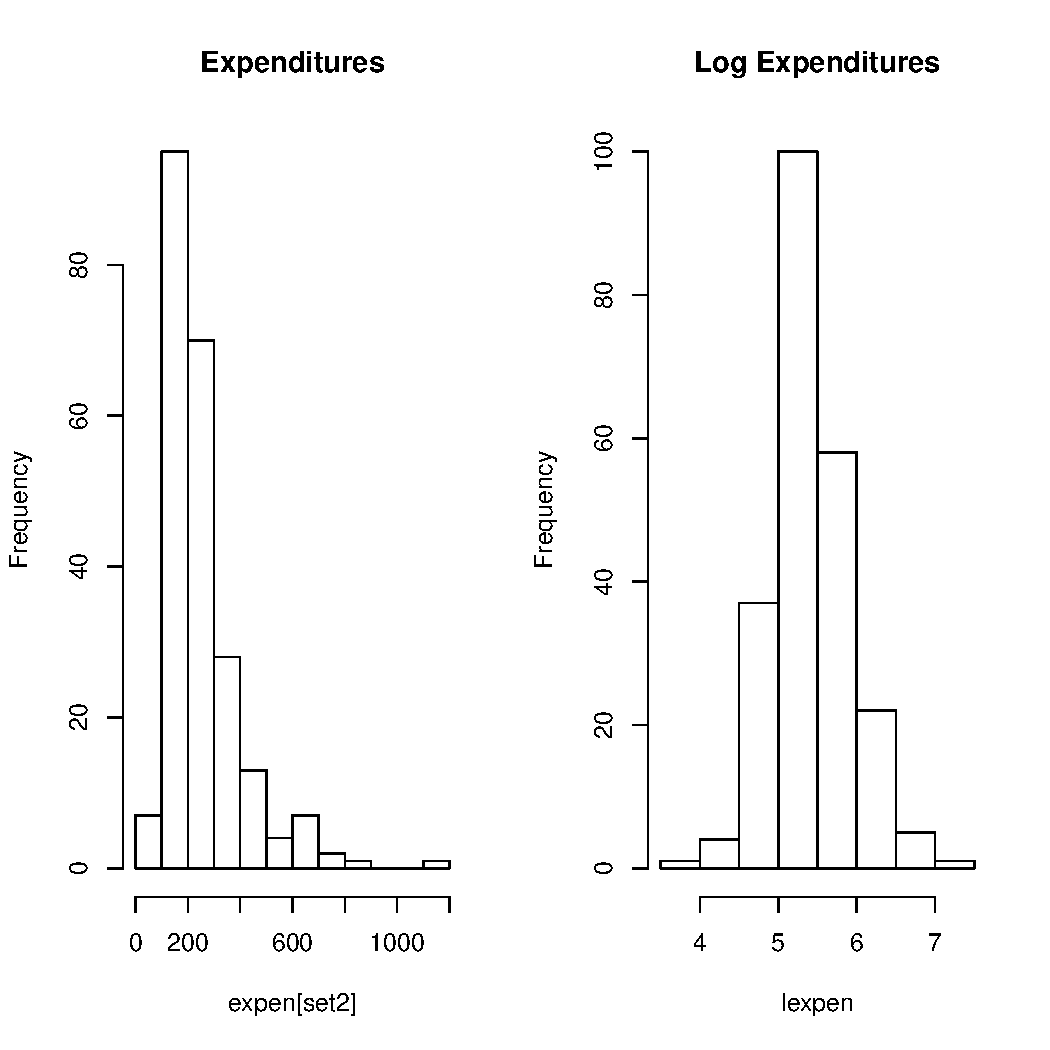
\includegraphics[width=0.5\linewidth,height=0.25\textheight]{figure/Log_transform_Response-1} 

\end{knitrout}
\end{center}
\end{figure}

\subsection{Model Fitting/Inferences}
\qquad After log transforming all variables, a correlation matrix should be examined. The correlation matrix showed that there were some highly correlated covariates shown in the appendix. Log pop and log density .8 correlation with log wealth and log income had .75 correlation. Such highly correlated variables could be dropped from the analysis due to parsimony, but a quickly glance at the Variance Inflation Factor table \ref{vif} shows no serious violations of numbers being greater than 7. With that said, the analysis kept all of its predictors.  

\qquad Using the function stepAIC, it was shown that the linear log log model was the best fit and modeled the data with the least amount of penalties. stepAIC is a function that fits possible models from the data given. Every possible model is given a penalty marker. The least amount of penalties, the better the model comes out to be. Looking at the stepAIC results were preferable compared to looking at coefficients from summary of the model and then manually dropping predictors one at a time before achieving the best fitted model.  This fit was reasonable because all, but the log-transformed density variable had less than a 0.05 p-value. Since the p-value of log-density wasn't that much higher than .05 and .05 was an arbitrary benchmark, the predictor log-density was left in. Further investigation into this model showed an influential point (obs 225) that was left in. While it is feasible to remove an outlier, it was kept in the analysis to account for extremities of the New York state. It is quite possible that observation 225 was Manhattan. With 914 observations, removing a single outlier probably will not change the model selection. Looking at figure \ref{cook}, the plot shows the predicted model with observation 225. The removal of observation 225 only slightly increases $R^2$  coefficient. $R^2$ is a statistical measure of how close the data are to the fitted regression line. I.e. how well the model explains the data set. Thus the outlier was retained in this analysis.

\begin{table}[h!]
  \begin{center}
    \caption{$95 \%$ Confidence Intervals of model's coefficients}
    \label{coefficients}
    \begin{tabular}{l|l|l} 
      \textbf{Coefficient} & \textbf{Lower Bound} & \textbf{Upper Bound}\\
      \hline
      Wealth   &  1.3 & 1.7 \\
      Pop       &  1.1 & 1.3 \\
      Pint       &  0.67 & 0.79 \\
      Dens      &  0.85 & 1.0\\
      Income  &   1.1 & 1.7 \\
      Growr    & 0.95 & 0.99 \\
      
    \end{tabular}
  \end{center}
\end{table}

\qquad From the model, expenditures by Warwick and Monroe can be predicted for the years 1992, 2005, and 2025. Those predicted expenditure values can be seen in table \ref{predictions}. These predictions should be kept in the minds of the city councils of Monroe and Warwick when they create annual budgets. In addition, the coefficients of each predictor can be found in table \ref{coefficients}. While it may look like the prediction intervals and estimated expenditures for Monroe remain fairly constant, the unrounded figures in the table within the appendix shows that there are slight increases over time. This may be due to Monroe being a small town. 
\begin{table}[h!]
  \begin{center}
    \caption{$95 \%$ Predictions Intervals of Warwick and Monroe Expenditures}
    \label{predictions}
    \begin{tabular}{c | c | c | c | c} \hline
      \textbf{Town} & \textbf{Year} & \textbf{Expen Est.} & \textbf{Lower Bound} & \textbf{Upper Bound}\\
      \hline
     Warwick & 1992 & 250 & 130 & 460 \\
                  & 2005 & 270 & 140 & 500 \\
                  & 2025 & 280 & 150 & 520 \\
                  \hline
	Monroe & 1992 & 250 & 130 & 460 \\
		     & 2005 & 250 & 140 & 470 \\
		     & 2025 & 250 & 140 & 470 \\
      
    \end{tabular}
  \end{center}
\end{table}

\begin{figure}
  \begin{center}
    \caption{Cook's Distance}
      \label{cook}
\begin{knitrout}
\definecolor{shadecolor}{rgb}{0.969, 0.969, 0.969}\color{fgcolor}
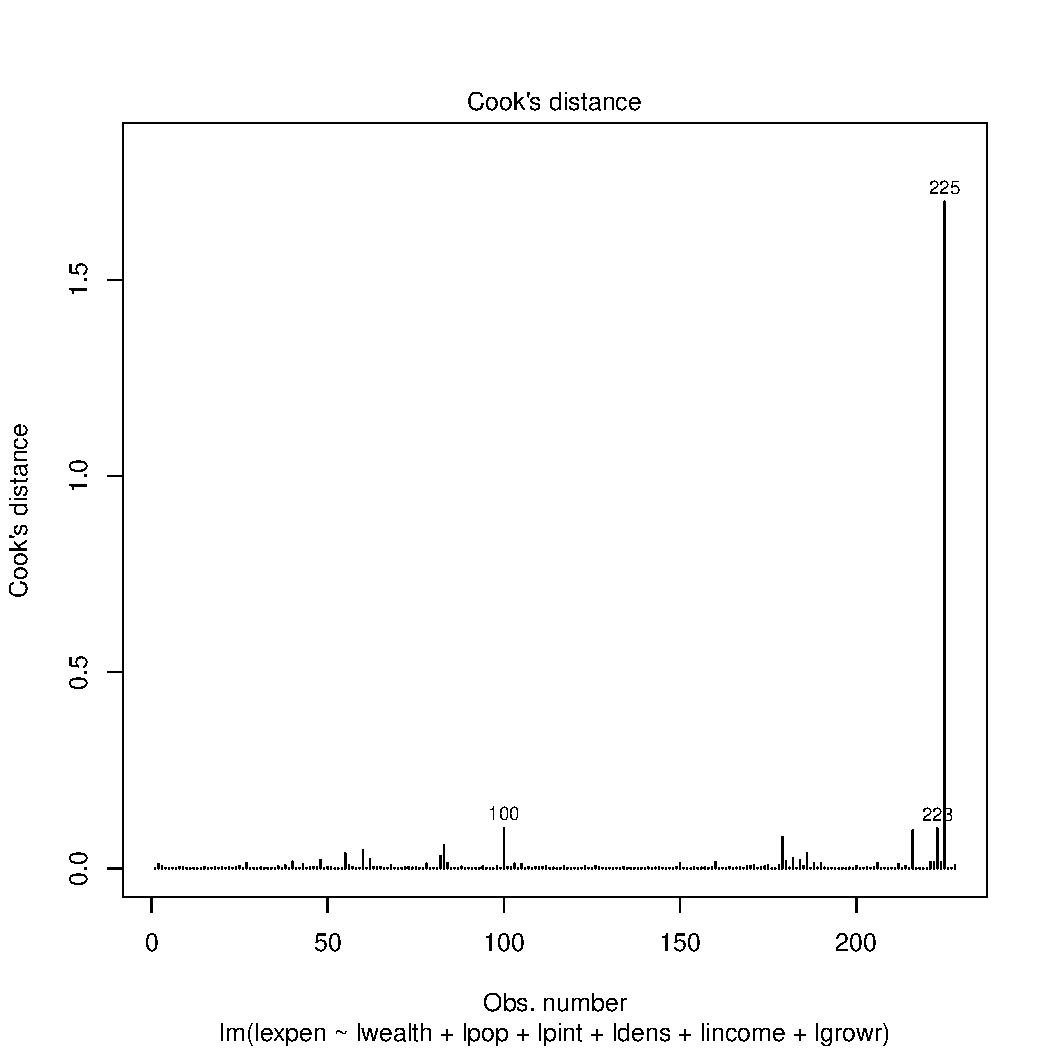
\includegraphics[width=0.4\linewidth]{figure/Cooks_Distance-1} 

\end{knitrout}
\end{center}
\end{figure}

\section{Conclusion}
\qquad In this analysis, it has shown that the expenditures of the New York municipalities Warwick and Monroe will most likely increase due to proposed construction of new housing projects. The two towns should look for methods to increase funds whether it be increasing property tax, increasing sales tax, or another method. Table \ref{predictions} has shown positive linear trend in expenditures for both towns. Warwick should find sources of revenue quicker than Monroe due to its ever increasing expenditures.

\qquad This analysis was limited in three ways. The first way was that the outlier was not taken out of the dataset even though it was looked at. $R^2$ may have increased by .05 without the outlier, but the model would have stay the same either way. Second, the analysis stuck to a linear log log model. There were a couple of predictors that were worth examining at a higher power. But not having variables log transformed would have prove disastrous. The last limitation was that the data was subsetted (log(pop) $>$ 8.3 \& log(dens) $>$ 4.5), thus data set with log(pop) $<$ 8.3 and log(dens) $<$ 4.5 was not considered. Presently, it is not clear why a subset of that nature should be looked at, but that data set may hold valuable information for Warwick and Monroe. For the future, these three limitations could be explored, but for now, this analysis should suffice. 

\qquad Since there is data on 1992 and 2005, it is possible to compare those actual values to the analysis' predicted values. It would be very interesting to see if those values lined up. If the values are no where close, then another model must be considered. In addition, would this model hold up to states similar to New York? With a little further investigation, surely, that question can be answered. 

%
\newpage
\noindent \Large{{\bf Appendix A: Auxiliary Graphics and Tables}}

%
\begin{figure}
\caption{BoxCox Transformation of Response Variable}
\begin{knitrout}
\definecolor{shadecolor}{rgb}{0.969, 0.969, 0.969}\color{fgcolor}
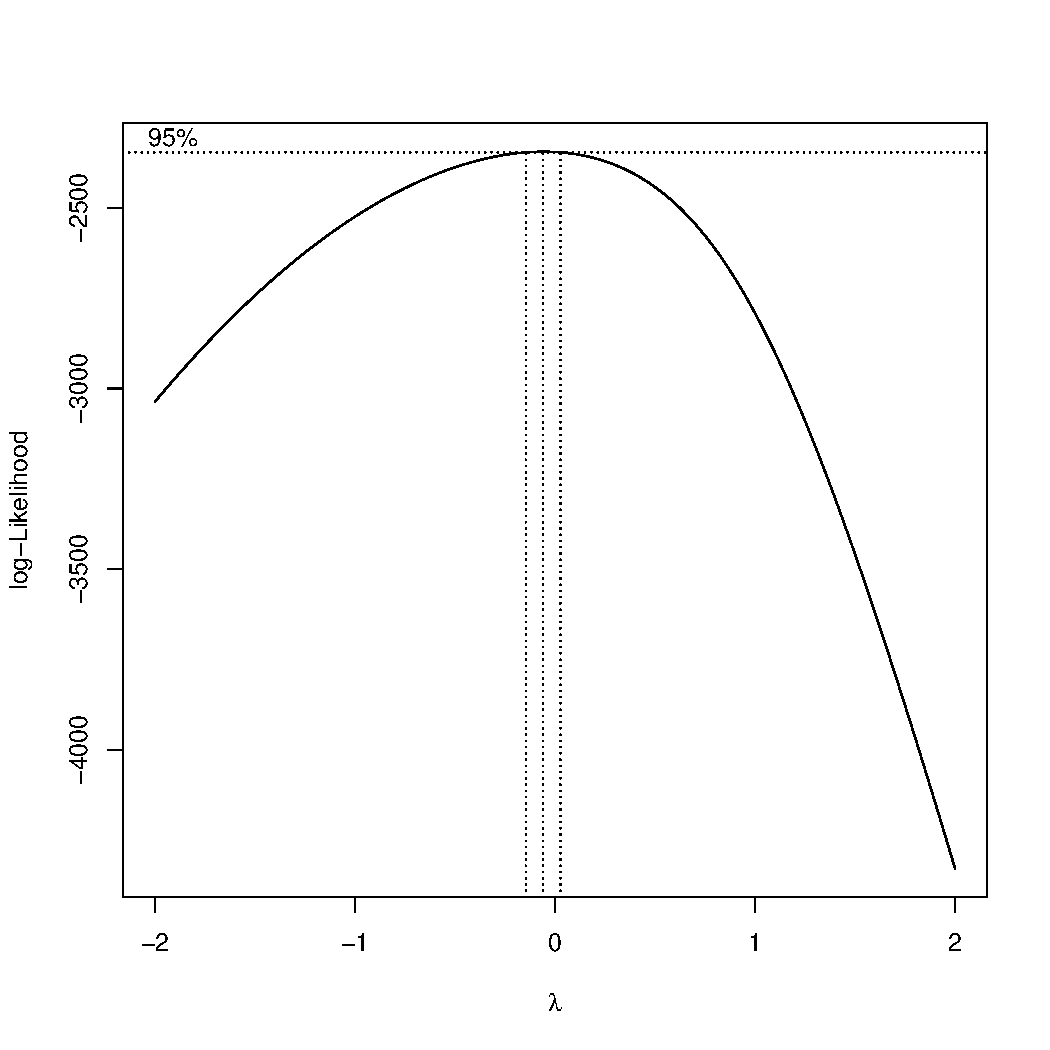
\includegraphics[width=\maxwidth,height=0.5\textheight]{figure/BoxCox_plot-1} 
\begin{kframe}\begin{verbatim}
## [1] -0.06060606
\end{verbatim}
\end{kframe}
\end{knitrout}
\end{figure}
%
\begin{figure}
\begin{center}
\caption{Homoscedasticity}
\label{residuals}
\begin{knitrout}
\definecolor{shadecolor}{rgb}{0.969, 0.969, 0.969}\color{fgcolor}
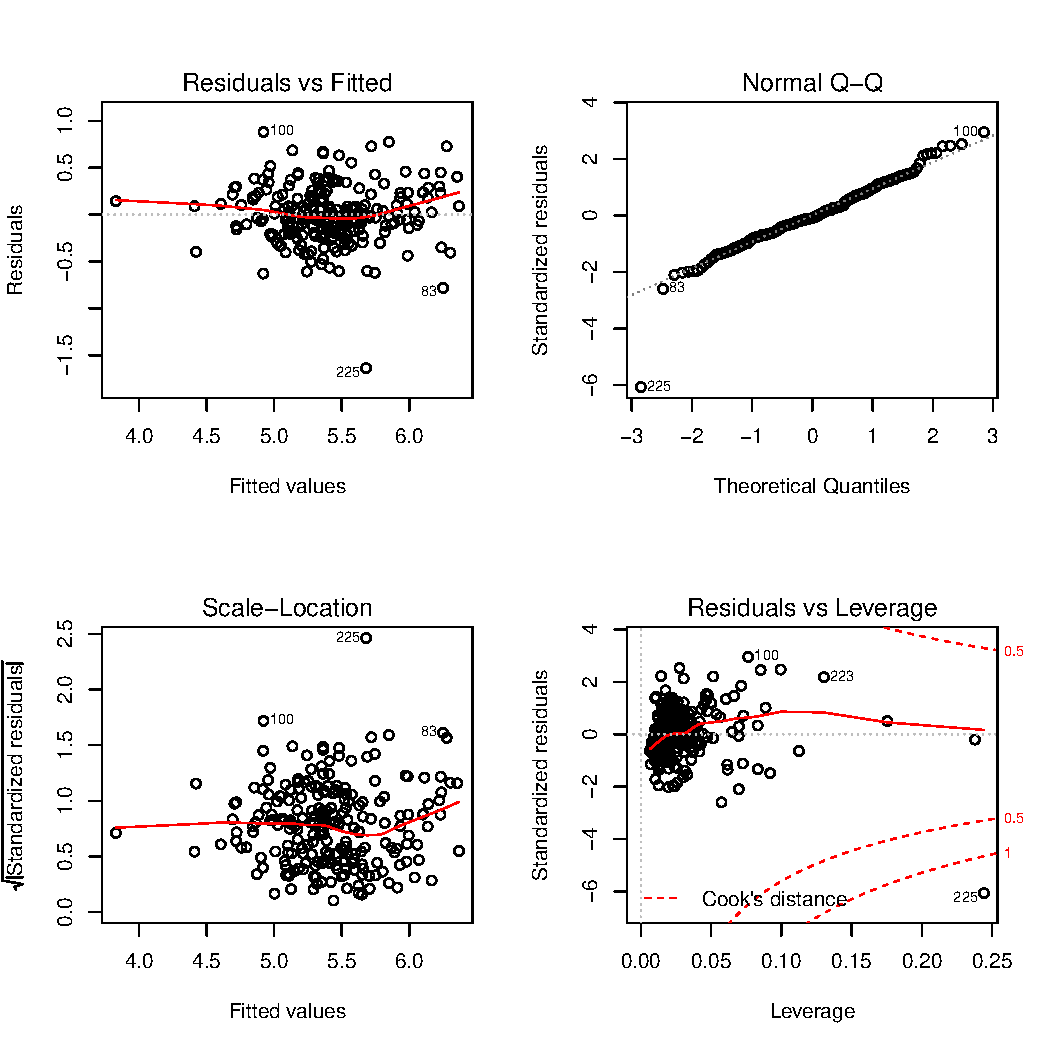
\includegraphics[width=\maxwidth]{figure/Homoscedasticity-1} 

\end{knitrout}
\end{center}
\end{figure}
%

\begin{knitrout}
\definecolor{shadecolor}{rgb}{0.969, 0.969, 0.969}\color{fgcolor}\begin{kframe}


{\ttfamily\noindent\itshape\color{messagecolor}{\#\# corrplot 0.84 loaded}}\end{kframe}
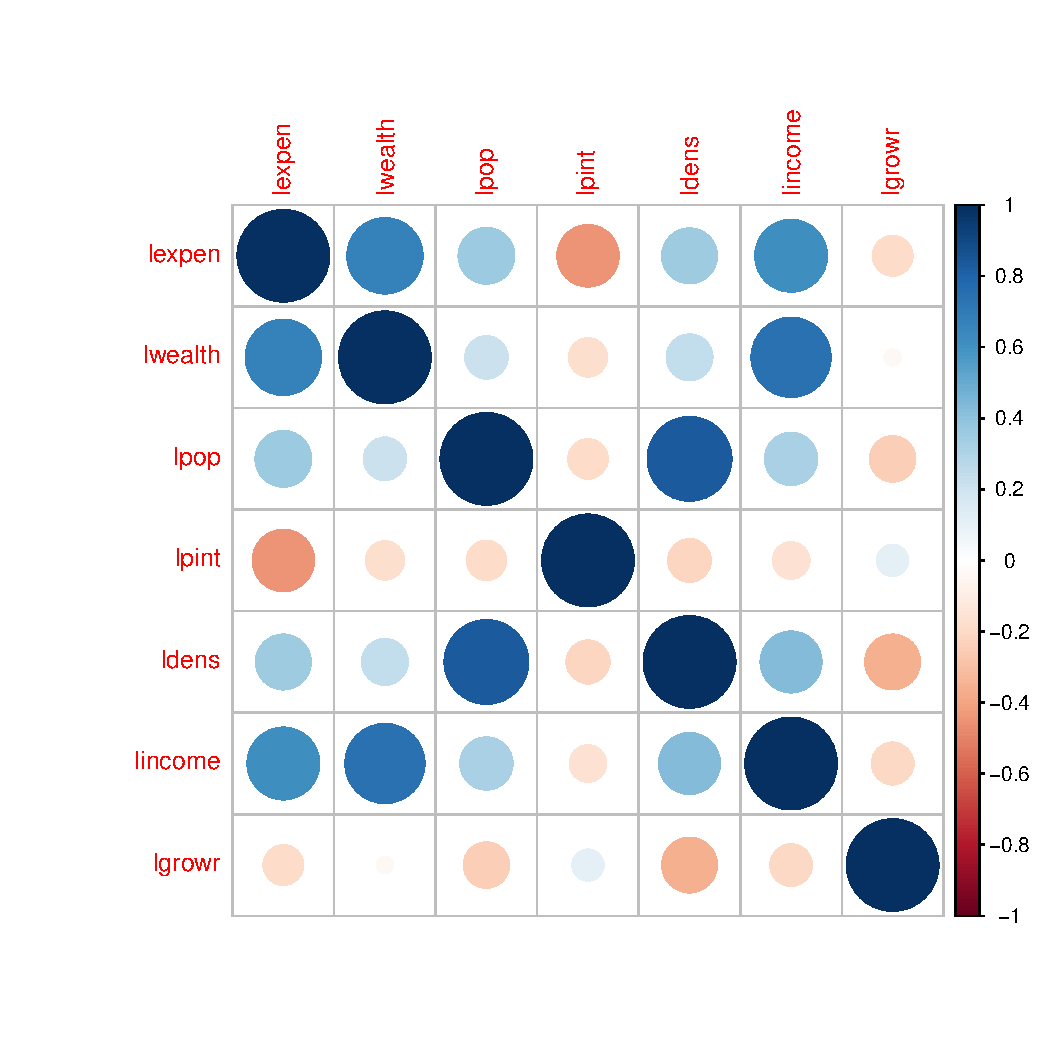
\includegraphics[width=\maxwidth]{figure/Correaltion_Matrix-1} 

\end{knitrout}

%
\begin{figure}
  \begin{center}
    \caption{Histograms of Not Transformed Predictors}
      \label{regular}
\begin{knitrout}
\definecolor{shadecolor}{rgb}{0.969, 0.969, 0.969}\color{fgcolor}
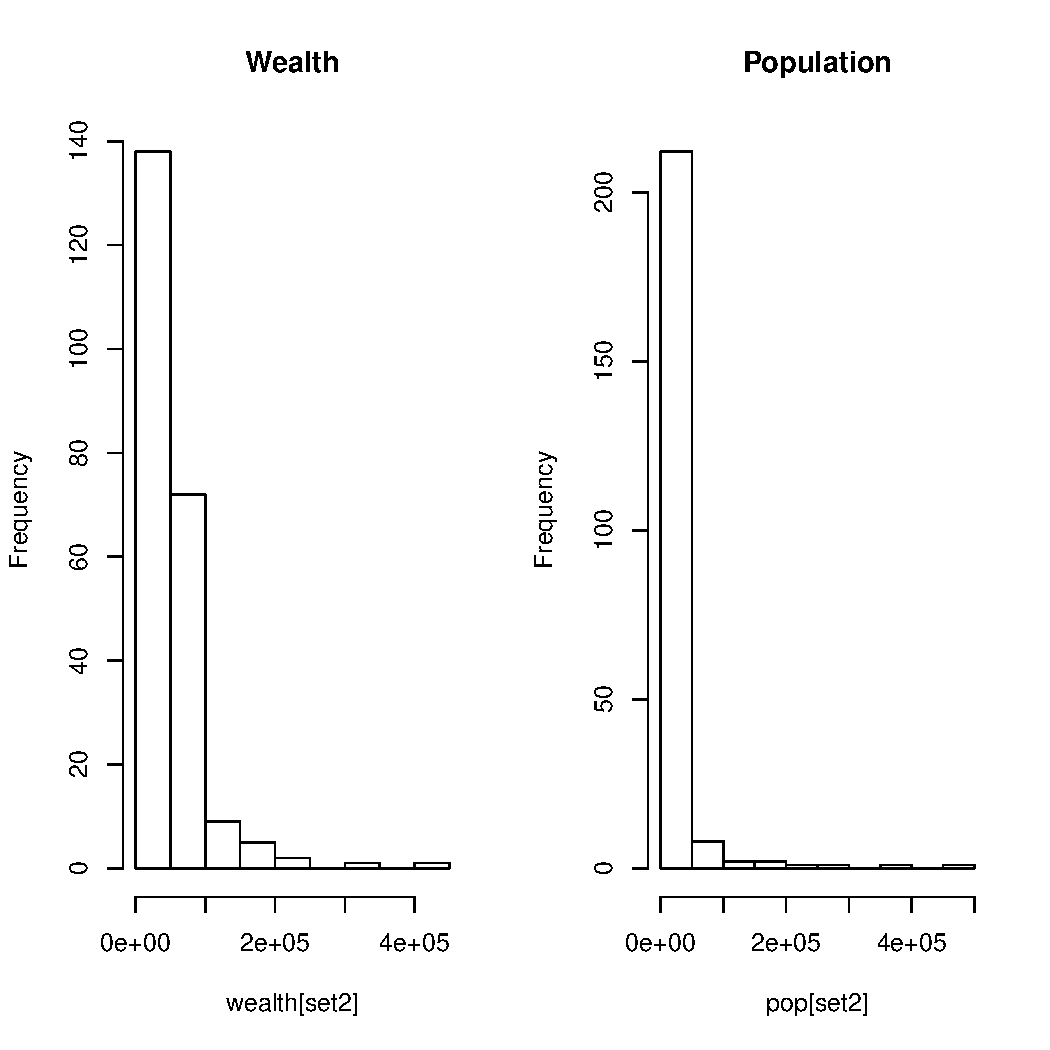
\includegraphics[width=\maxwidth,height=0.3\textheight]{figure/Not_Transformed_Predictors-1} 

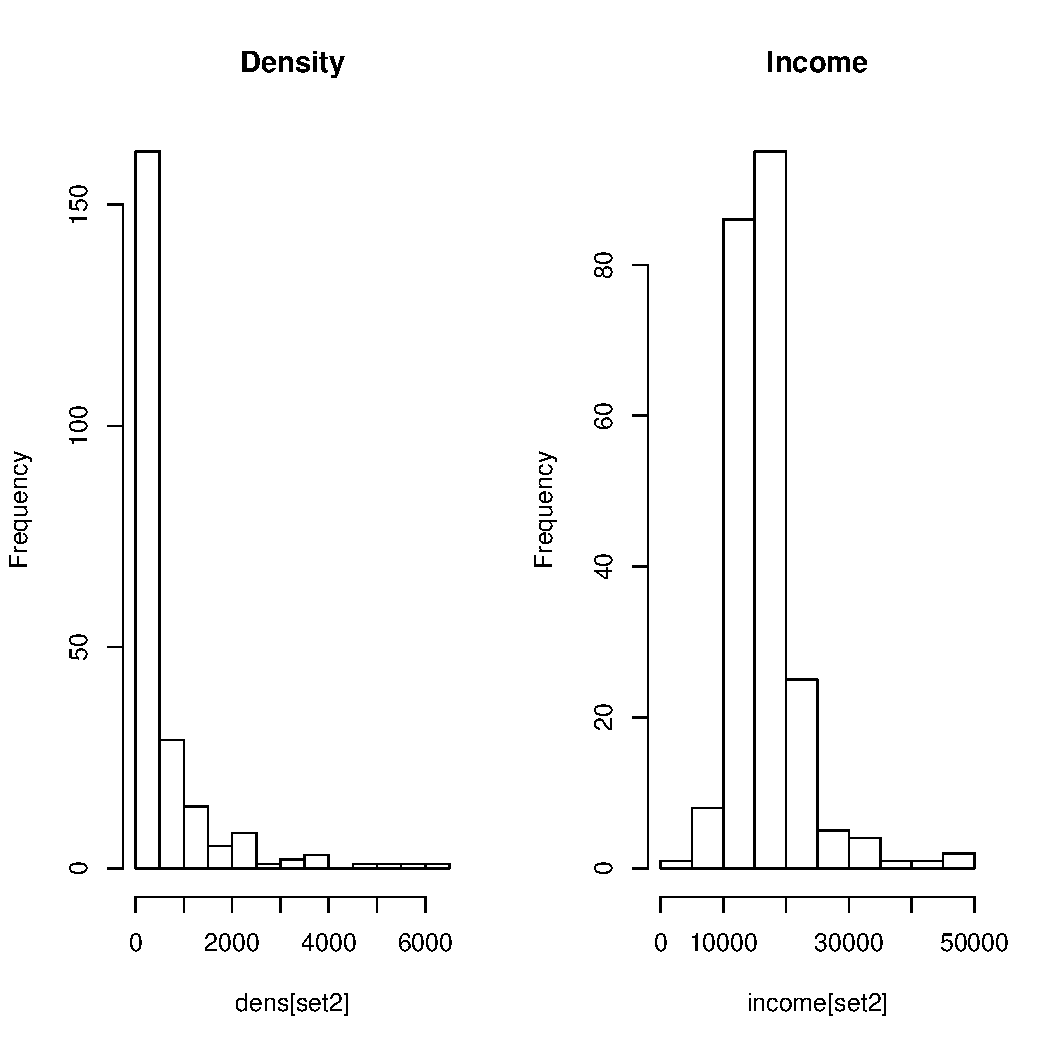
\includegraphics[width=\maxwidth,height=0.3\textheight]{figure/Not_Transformed_Predictors-2} 

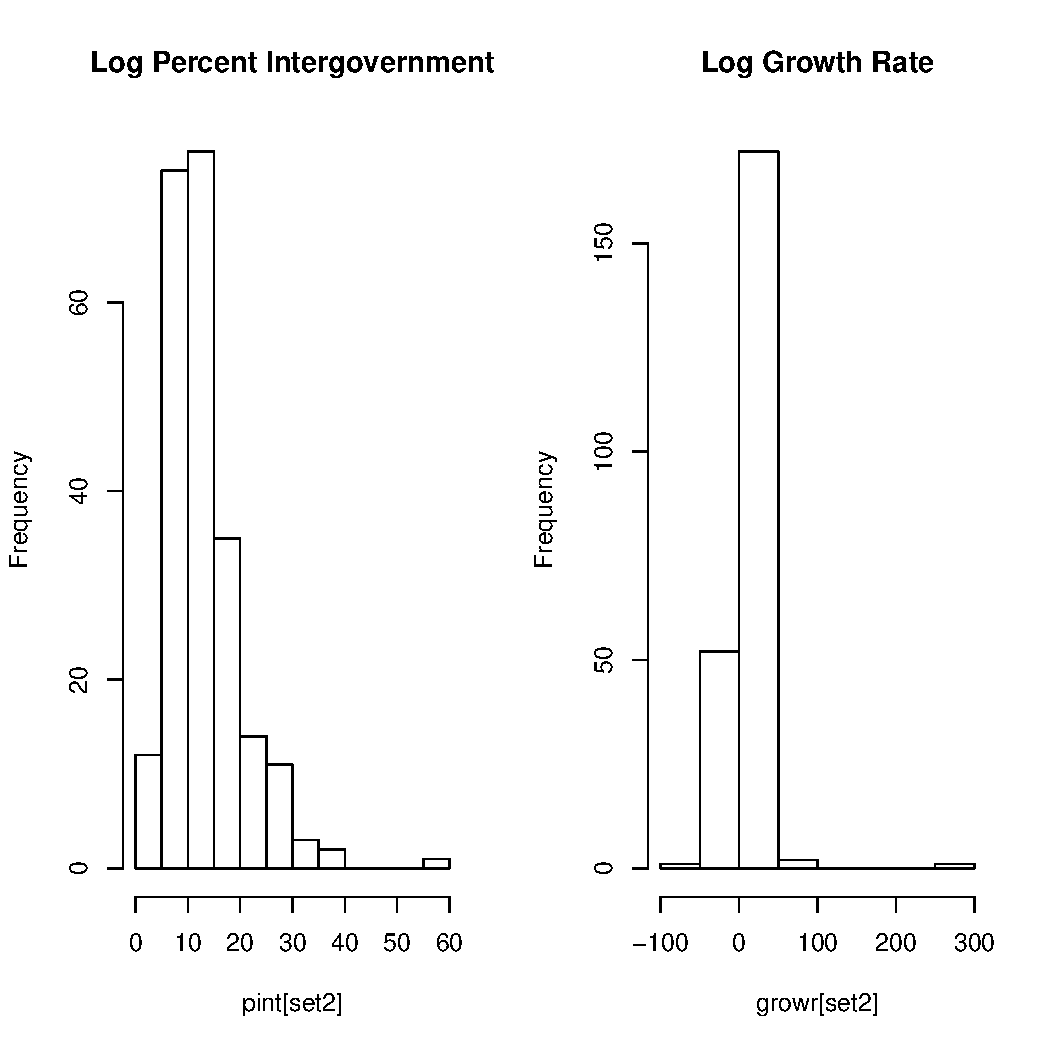
\includegraphics[width=\maxwidth,height=0.3\textheight]{figure/Not_Transformed_Predictors-3} 

\end{knitrout}
  \end{center}
\end{figure}
%
\begin{figure}
  \begin{center}
    \caption{Histograms of Log Transformed Predictors}
      \label{transformed}
\begin{knitrout}
\definecolor{shadecolor}{rgb}{0.969, 0.969, 0.969}\color{fgcolor}
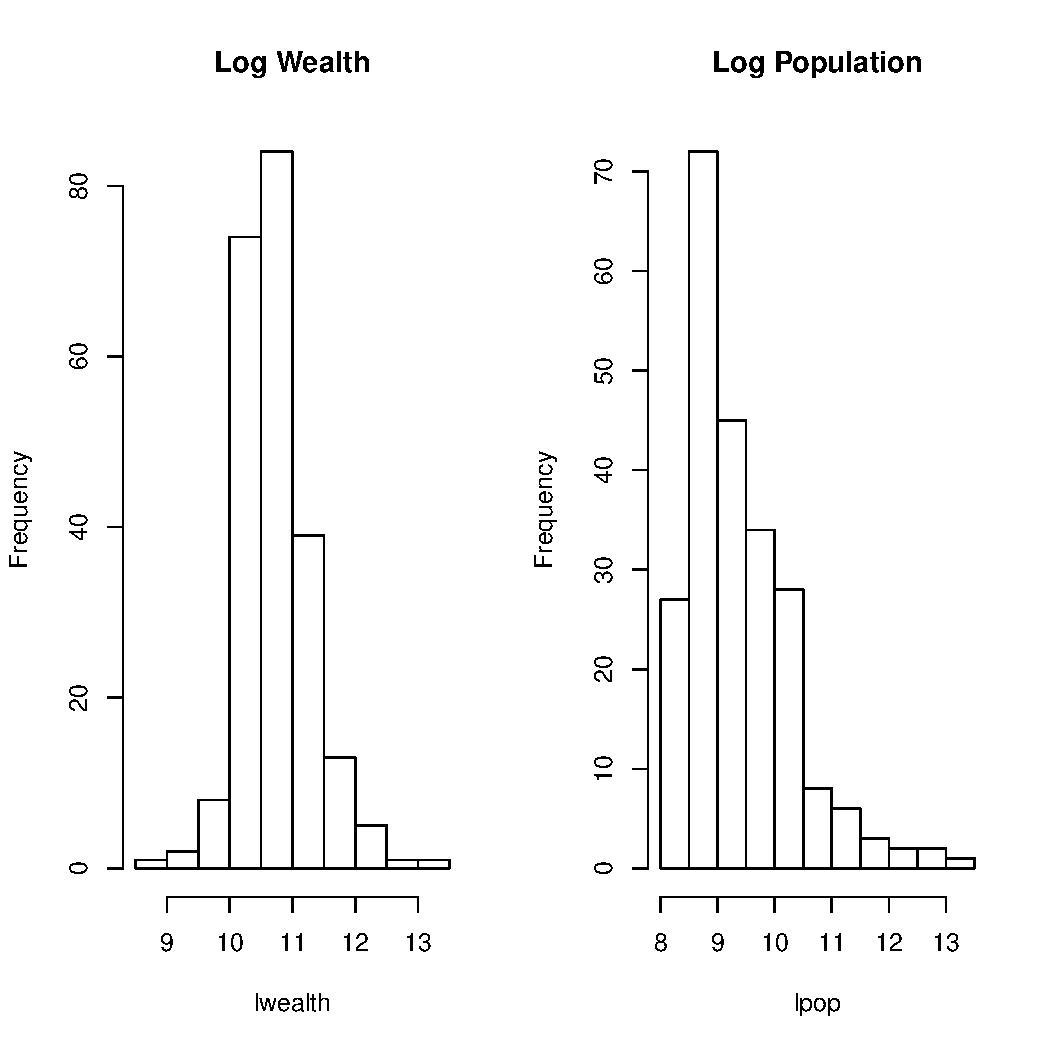
\includegraphics[width=\maxwidth,height=0.3\textheight]{figure/Log_Transformed_Predictors-1} 

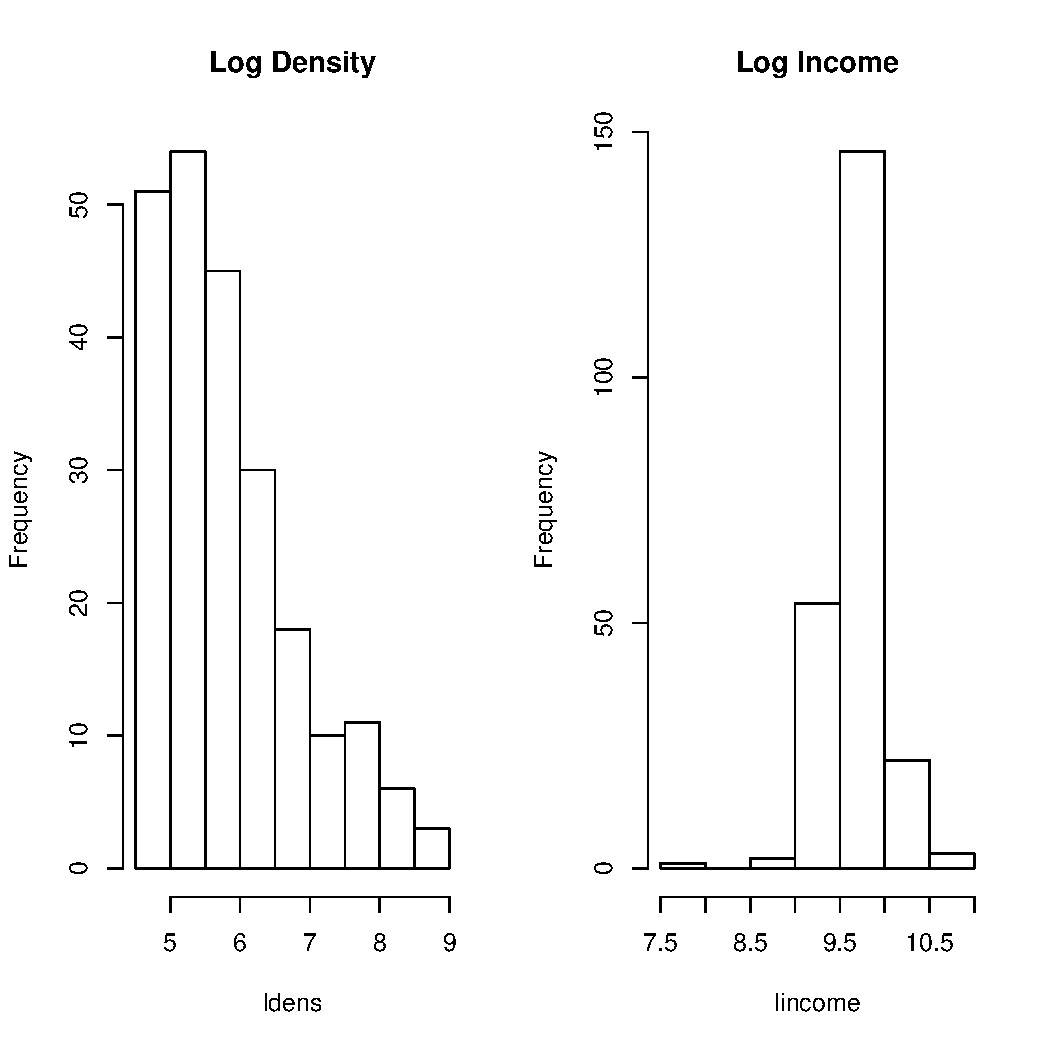
\includegraphics[width=\maxwidth,height=0.3\textheight]{figure/Log_Transformed_Predictors-2} 

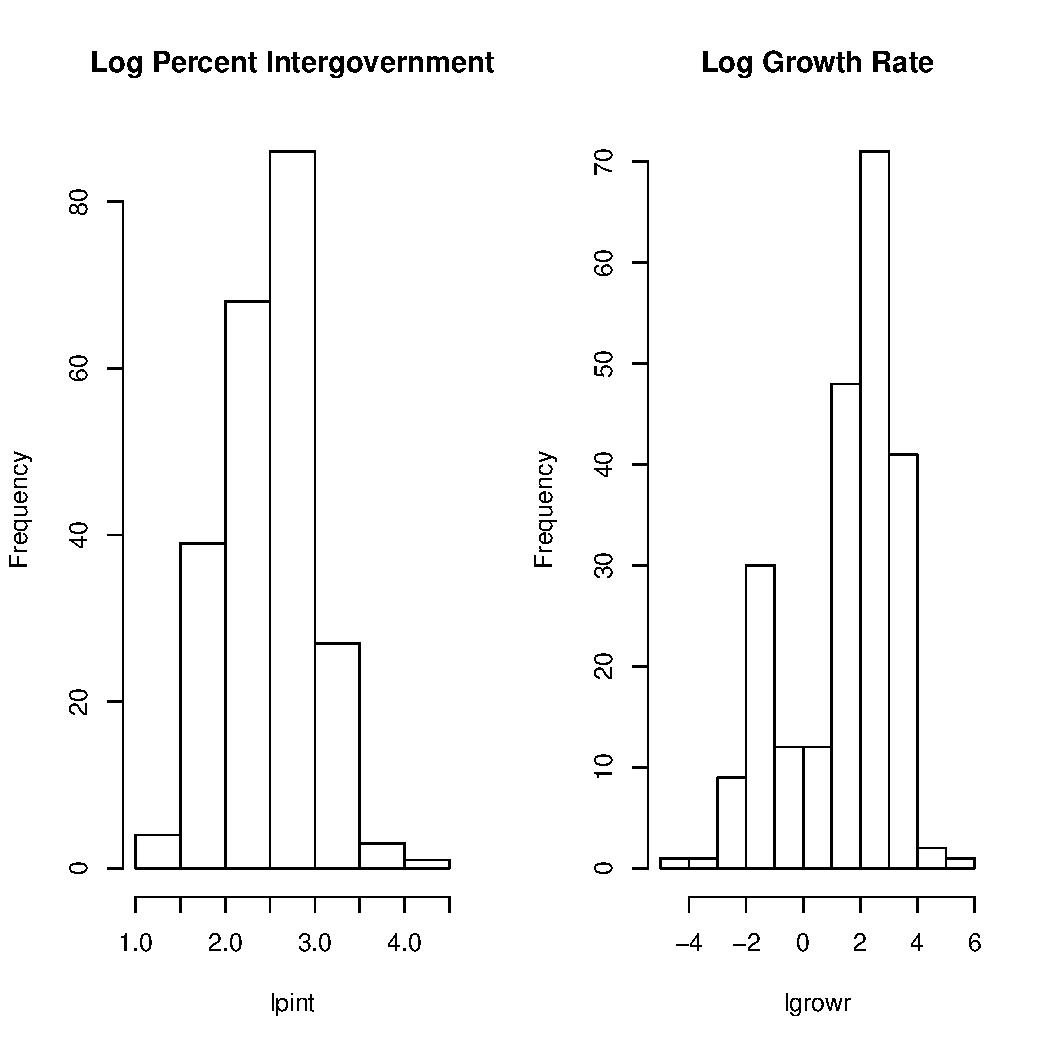
\includegraphics[width=\maxwidth,height=0.3\textheight]{figure/Log_Transformed_Predictors-3} 

\end{knitrout}
  \end{center}
\end{figure}
%
\begin{figure}
\begin{center}
\caption{Log Expenditures vs Covariates}
\label{scatterplots}
\begin{knitrout}
\definecolor{shadecolor}{rgb}{0.969, 0.969, 0.969}\color{fgcolor}
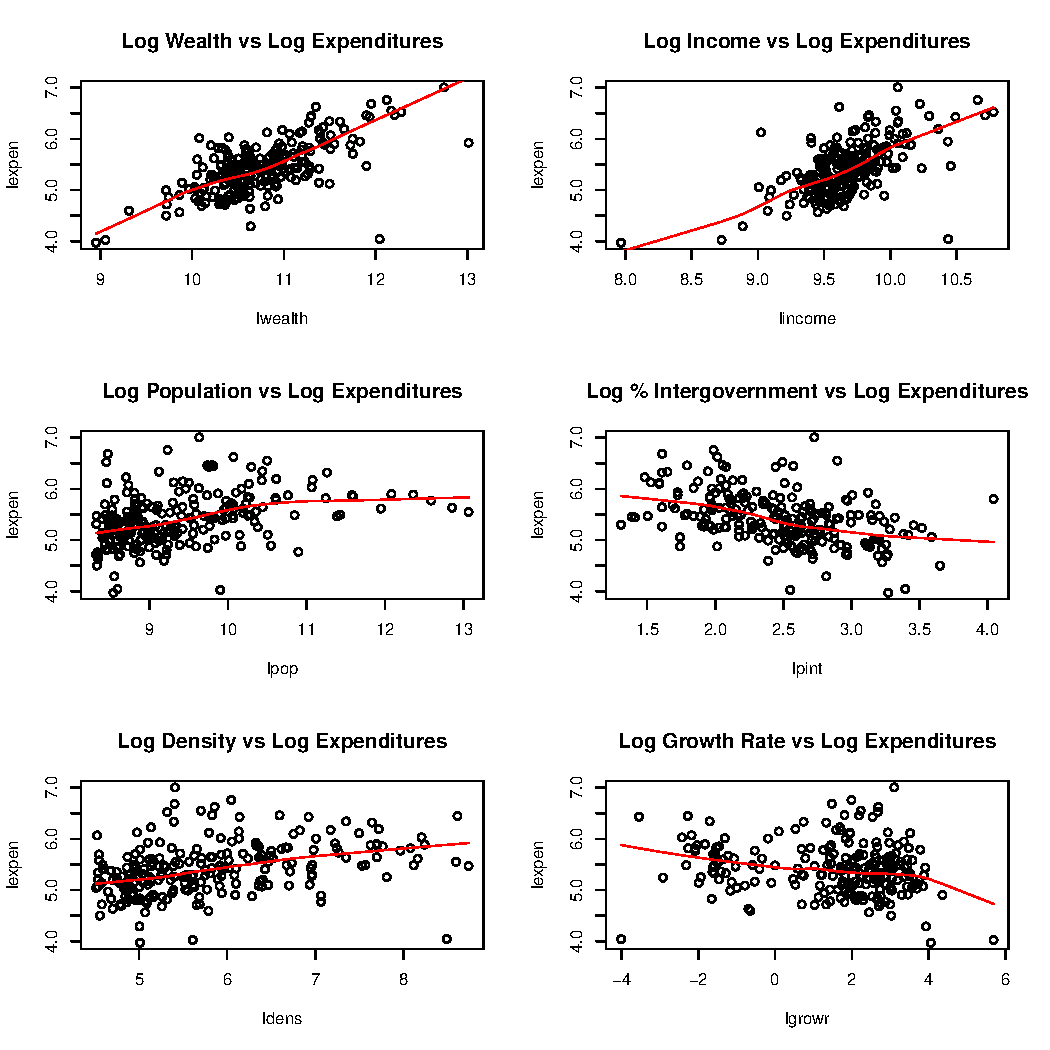
\includegraphics[width=0.7\linewidth]{figure/Expend_vs_Covariates-1} 

\end{knitrout}
\end{center}
\end{figure}
%

%
\begin{table}[h!]
  \begin{center}
    \caption{Variance Inflation Factor}
    \label{vif}
    \begin{tabular}{c | c | c | c | c | c} \hline
      \textbf{Lwealth} & \textbf{Lpop} & \textbf{Lpint} & \textbf{Ldens} & \textbf{Lincome}& \textbf{Lgrowr}\\
      \hline
     2.4 & 3.4 & 1.1 & 4.0 & 2.8 & 1.2 \\
    \end{tabular}
    \end{center}
\end{table}
%
\begin{table}[h!]
  \begin{center}
    \caption{$95 \%$ Confidence Intervals of model's coefficients}
       \begin{tabular}{l|l|l} 
      \textbf{Coefficient} & \textbf{Lower Bound} & \textbf{Upper Bound}\\
      \hline
      (Intercept) & 0.03791628 & 0.7578978 \\
Lwealth     & 1.33904808 & 1.6666506 \\
Lpop        & 1.06202032 & 1.2521650 \\
Lpint       & 0.67044390 & 0.7946076 \\
Ldens       & 0.85051014 & 1.0037347 \\
Lincome     & 1.07781031 & 1.6605132 \\
Lgrowr      & 0.95239659 & 0.9989585 \\
      
    \end{tabular}
  \end{center}
\end{table}
                
\begin{table}[h!]
  \begin{center}
    \caption{$95 \%$ Predictions Intervals of Warwick and Monroe Expenditures}
    
    \begin{tabular}{c | c | c | c | c} \hline
      \textbf{Town} & \textbf{Year} & \textbf{Expen Est.} & \textbf{Lower Bound} & \textbf{Upper Bound}\\
      \hline
     Warwick & 1992 & 248.2336 & 133.1536 & 462.773 \\
             & 2005 & 268.8325 & 144.0641 & 501.658 \\
             & 2025 & 277.8198 & 148.6064 & 519.3843 \\
                  \hline
	Monroe & 1992 & 248.0169 & 133.4198 & 461.0441 \\
		     & 2005 & 253.7929 & 136.4834 & 471.9316 \\
		     & 2025 & 254.4445 & 136.7075 & 473.5805 \\
      
    \end{tabular}
  \end{center}
\end{table}


\newpage
\noindent \Large{{\bf Appendix B: R Code}}
\lstinputlisting[language=R, caption = Warwick and Monroe]{NYexpen.R}
\end{document}
